\documentclass[apectratio=169]{beamer}
\usetheme{metropolis}           % Use metropolis theme
% For PDFs
\newcommand{\myast}{\ensuremath{^{\ast}}}
\newcommand{\mydagger}{\ensuremath{^{\dagger}}}
\usepackage{pdfpages}
\usepackage{minted}
\usepackage{siunitx}
\title{Enabling Ambient Backscatter\\
Using a Low-Cost Software Defined Radio}
\subtitle{Saving Energy/Low Power Communications}
\date{\vspace{1em}
\today}
\author{Maximilian Stiefel\myast, Elmar van Rijnswou\myast\\Carlos Pérez-Penichet\myast, Ambuj Varshney\myast, Christian Rohner\myast and Thiemo Voigt \mydagger
\\\myast Uppsala University
\\\mydagger Uppsala University and RISE SICS
}
\institute{13th Swedish National Computer Networking Workshop}
\begin{document}
  \maketitle

\begin{frame}{Table Of Contents}
  \setbeamertemplate{section in toc}[sections numbered]
  \tableofcontents[hideallsubsections]
\end{frame}

\section{Introduction}
\begin{frame}{What is Backscattering? (1)}
	\begin{figure}[H]	
		\centering
		\only<1>{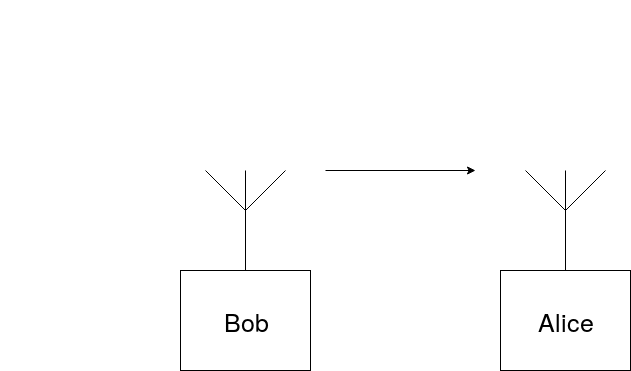
\includegraphics[width=0.8\textwidth]{./fig/backscatter1}}
		\only<2>{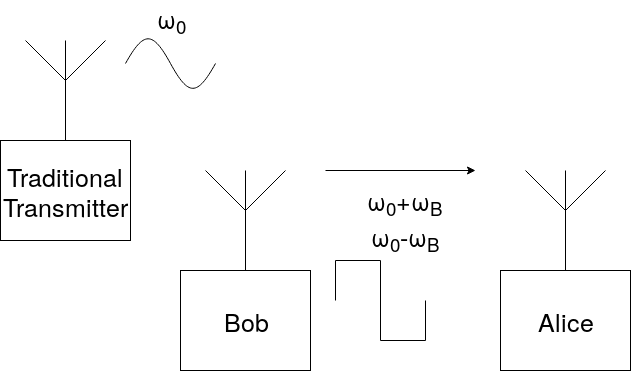
\includegraphics[width=0.8\textwidth]{./fig/backscatter2}}
		\caption{Simplest form of backscattering.}
	\end{figure}
\end{frame}

\begin{frame}{What is Backscattering? (2)}
	\only<1->{\begin{figure}[H]	
		\centering
		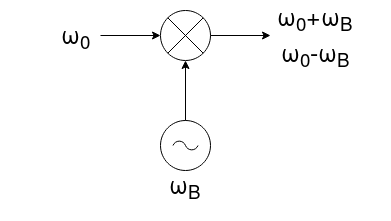
\includegraphics[width=0.6\textwidth]{./fig/mixer}
		\caption{Classical communications engineering element: The mixer.}
	\end{figure}}
	\only<2->{\begin{equation}
	2\sin(f_c t) \sin(\Delta f t) = \cos[(f_c + \Delta f)t] - \cos[(f_c - \Delta f) t]
	\label{eq:mixing}
	\end{equation}}

\end{frame}

\begin{frame}{What is Backscattering? (3)}
	\only<1->{\begin{figure}[H]	
		\centering
		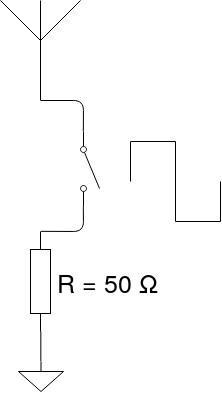
\includegraphics[height=0.5\textheight]{./fig/rfswitch}
		\caption{\SI{50}{\ohm} connected to a RF switch do the trick.}
	\end{figure}}
	\only<2->{
		\begin{equation}
			\Gamma = \frac{Z_L - Z_A}{Z_L + Z_A}
		\end{equation}
	}
\end{frame}

\begin{frame}{Why Backscattering?}
	\begin{itemize}
		\item<1-> Ultra-low power wireless transmissions by reflecting/absorbing EM waves (in orders of \SI{}{\micro\watt}) \cite{liu_ambient_2013}
		\item<2-> Leverage existing signals such as coming from WiFi \cite{hitchhike,kellogg2015wi} or TV towers \cite{liu_ambient_2013,parks_turbocharging_2014}
		\item<3-> Mechanism of choice to network devices operating on harvested energy
		\item<4-> Communication frontends are much simpler, smaller and cheaper, than traditional RF frontends
	\end{itemize}
\end{frame}

\section{Background}
\begin{frame}{What is Backscattering?}
	\begin{minipage}{0.47\textwidth}
	\begin{itemize}
		\item Different backscattering research has already been done (e.g. \cite{Vincent})
		\item Also a lot of things about the RTL2832U can be found (e.g. \cite{Ana}) 
	\end{itemize}
	\end{minipage}
	\hfill
	\begin{minipage}{0.47\textwidth}
	\begin{figure}[H]	
		\centering
		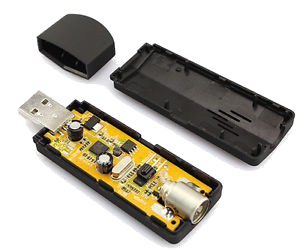
\includegraphics[width=1\textwidth]{./fig/rtlsdr}
		\caption{The IQ demodulator RTL2832U is available for less than 10 \$. Source: Ebay}
	\end{figure}
	\end{minipage}
\end{frame}
	
\begin{frame}{Background And Literature (2)}
	\begin{figure}[H]	
		\centering
		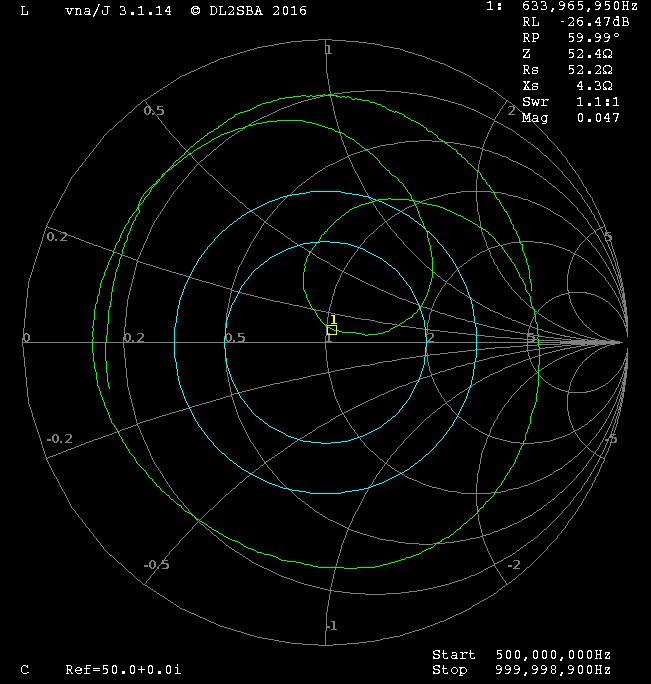
\includegraphics[height=0.75\textheight]{./fig/monopole_smith}
		\caption{Smitchart sweep of selfmade ground-plane antenna for 634 MHz (checkout \cite{Pozar}).}
	\end{figure}
\end{frame}

\begin{frame}{Background And Literature (3)}
	\begin{figure}[H]	
		\centering
		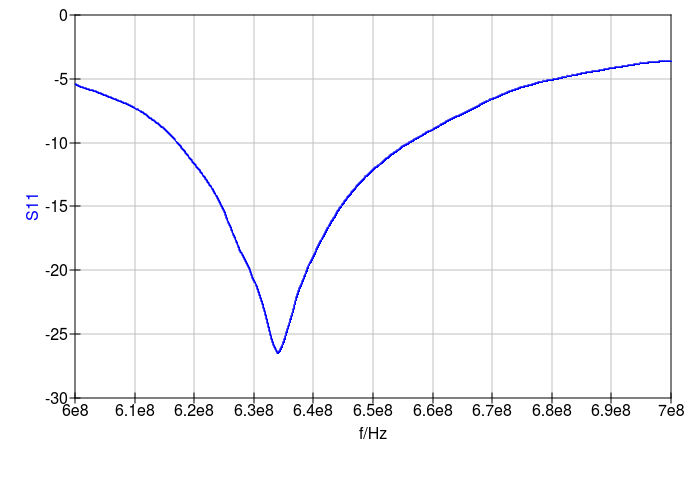
\includegraphics[height=0.75\textheight]{./fig/monopole_S11dB}
		\caption{S11 out of the S parameter file of the VNA plotted with Qucs.}
	\end{figure}
\end{frame}


\section{Design}
\begin{frame}{State Of The Project (1)}
	\begin{table}[]
	\centering
	\begin{tabular}{ll}
	\hline
	\textbf{Backscatter Tag}               &    \\\hline
	Manchester encoding                    &   \checkmark \\
	Weak error protection                  &   \checkmark\\
	Shifting by 2 MHz                      &   \checkmark\\
	Advanced frame design                  &   \checkmark\\
	\hline
	\textbf{Antenna}                       &    \\\hline
	Roughly tuned and matched              &    \checkmark\\\
	Mechanical stability                   &    \\
	Lumped elements tuning                 &    \\\hline
	\end{tabular}
	\caption{Backscatter tag and antenna}
	\end{table}
\end{frame}
\begin{frame}{State Of The Project (2)}
	\begin{table}[]
	\centering
	\begin{tabular}{ll}
	\hline
	\textbf{Receiver}                      &    \\\hline
	Signal processing                      &    \checkmark\\\
	Reception with certain bit error rate  &    \checkmark\\\
	Efficient infrastructure               &    \checkmark\\\
	Fast				       &    \\\hline
	\textbf{Measurements}                  &    \\\hline
	Processing and Measurement environment &    \checkmark\\\
	Massive amount of samples              &    \\\hline
	\end{tabular}
	\caption{Receiver and measurements}
	\end{table}
\end{frame}

\begin{frame}{State of the project (3)}
\begin{figure}[H]	
		\centering
		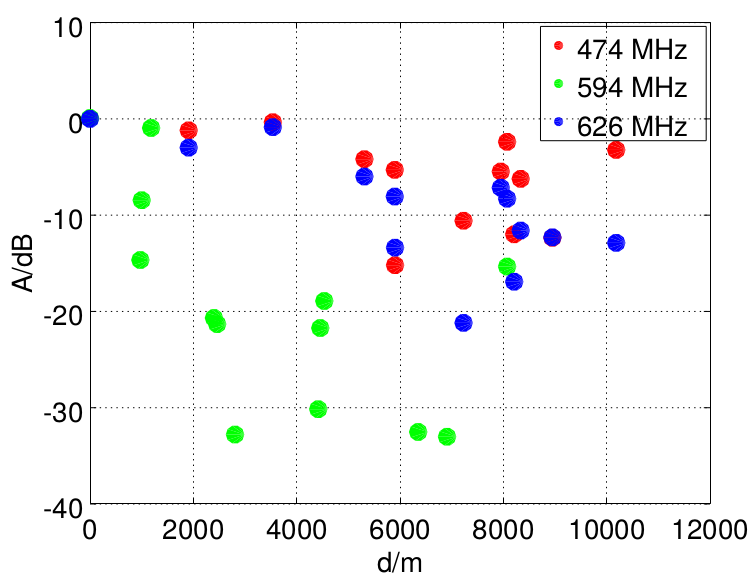
\includegraphics[height=0.75\textheight]{./fig/haversine}
		\caption{Signal strength depending on the distance of different frequencies.}
\end{figure}
\end{frame}

\begin{frame}[fragile]{State of the project (3)}
\begin{minted}[baselinestretch=1, fontsize=\tiny, linenos,frame=single,framesep=5pt]{Octave}
function d = haversine (lat1,lat2,lon1,lon2)
        R = 6371e3;                                                     % Earth radius
        rad = pi/180;

        phi1 = lat1*rad;
        phi2 = lat2*rad;
        dphi = (lat2-lat1)*rad;
        dlambda = (lon2-lon1)*rad;

        a = sin(dphi/2)*sin(dphi/2) + cos(phi1)*cos(phi2)*sin(dlambda/2)*sin(dlambda/2);
        c = 2*atan2(sqrt(a), sqrt(1-a));
        d = R*c;
endfunction;
\end{minted}
\end{frame}

\begin{frame}{State of the project (3)}
\begin{figure}[H]	
		\centering
		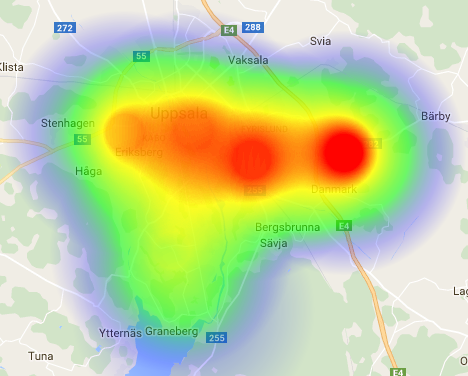
\includegraphics[height=0.75\textheight]{./fig/heatmap}
		\caption{Signal strength heatmap of 626 MHz signal.}
\end{figure}
\end{frame}

\begin{frame}{State Of The Project (4)}
	\only<1>{\begin{figure}[H]	
		\centering
		\includegraphics[height=0.7\textheight]{./fig/backscatter_arch_blank}
		\caption{System architecture of the receiver.}
	\end{figure}}
	\only<2>{\begin{figure}[H]	
		\centering
		\includegraphics[height=0.7\textheight]{./fig/backscatter_arch}
		\caption{System architecture of the receiver.}
	\end{figure}}
\end{frame}
 
\begin{frame}{State Of The Project (5)}
	\begin{figure}[H]	
		\centering
		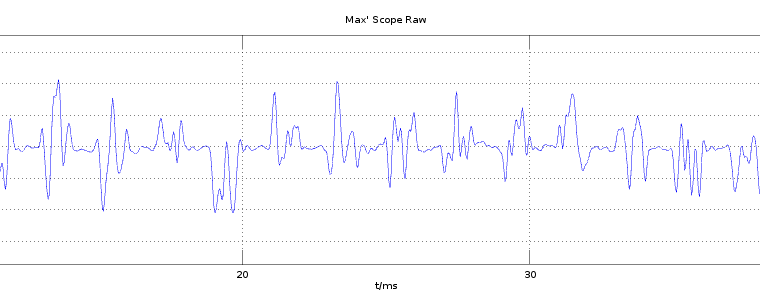
\includegraphics[height=0.5\textheight]{./fig/osci}
		\caption{Octave oscilloscope written for debugging purposes.}
	\end{figure}
\end{frame}

\section{Evaluation}
\begin{frame}{Conclusion}
\begin{itemize}
	\item Working receiver \checkmark
	\item Spectrum anlayzer based on the RTL2832U \checkmark 
	\item Working backscatter tag \checkmark
	\item Lot of help from the communication group \checkmark
\end{itemize}
\end{frame}

\begin{frame}{Outlook}
\begin{itemize}
	\item Reliable communication (e.g. hamming code)
	\item More advanced signal processing (e.g. oversampling) 
	\item Better (selfmade) antenna
	\item Other receiver hardware? 
\end{itemize}
\end{frame}

   	\begin{frame}{Contact Information}
        	\begin{center}
                \begin{table}[]
                        \begin{tabular}{ll}
                                E: & Elmar.Vanrijnswou.9818@student.uu.se \\
                             	E: & Maximilian.Stiefel.8233@student.uu.se\\
                        \end{tabular}
                \end{table}
                
\includegraphics[width=0.05\textwidth]{./fig/github} \hspace{0.1cm} \url{https://github.com/m3x1m0m}\\
        	\end{center}
        	\begin{figure}
                	
\includegraphics[width=0.3\textwidth]{./fig/logo}
        	\end{figure}
  	\end{frame}

\begin{frame}[standout]
	Happy Coding :) 
\end{frame}

\begin{frame}[allowframebreaks]{References}

  \bibliography{presentation}
  \bibliographystyle{abbrv}

\end{frame}

\end{document}
